\documentclass{article}

% Pretty much all of the ams maths packages
\usepackage{amsmath,amsthm,amssymb,amsfonts}

% Set up some environments
\newtheorem{thm}{Theorem}[section]
\newtheorem{lem}[thm]{Lemma}
\newtheorem{dfn}{Definition}[section]
\theoremstyle{dfn}
\newtheorem{alg}{Algorithm}[section]
\numberwithin{equation}{section}
\numberwithin{figure}{section}

% Pretty much all of the algorithms packages
\usepackage{algorithmicx,algpseudocode}

% Allows you to manipulate the page a bit
\usepackage[margin=1in]{geometry}

% Pulls the page out a bit - makes it look better (in my opinion)
\usepackage{a4wide}

% Allows inclusion of graphics easily and configurably
\usepackage{graphicx}

% Provides ways to make nice looking tables
\usepackage{booktabs}

% Allows you to rotate tables and figures
\usepackage{rotating}

% Allows shading of table cells
\usepackage{colortbl}
% Define a simple command to use at the start of a table row to make it have a shaded background
\newcommand{\gray}{\rowcolor[gray]{.9}}

\usepackage{textcomp}

% Provides commands to make subfigures (figures with (a), (b) and (c))
\usepackage{subfigure}

% Typesets URLs sensibly - with tt font, clickable in PDFs, and not breaking across lines
\usepackage{url}

% Makes references hyperlinks in PDF output
\usepackage{hyperref}

% Provides ways to include syntax-highlighted source code
\usepackage{listings}
\lstset{frame=single, basicstyle=\ttfamily}

% Provides good access to colours
\usepackage{color}
\usepackage{xcolor}

% Simple command I defined to allow me to mark TODO items in red
\newcommand{\todo}[1] {\textbf{\textcolor{red}{#1}}}

% Command for vector, matrix, tensor names
\renewcommand{\vec}[1] {\mathbf{#1}}
%\usepackage{esvect}
\newcommand{\Mat}[1] {\mathbf{#1}}
\newcommand{\Ten}[1] {\mathbf{\mathcal{#1}}}
\newcommand{\Pop}[1] {\mathcal{#1}}

% Command for important sets
\newcommand{\F} {\mathbb{F}}
\newcommand{\N} {\mathbb{N}}

% Allows fancy stuff in the page header
\usepackage{fancyhdr}
\pagestyle{fancy}

% Vastly improves the standard formatting of captions
\usepackage[margin=10pt,font=small,labelfont=bf, labelsep=endash]{caption}

% Standard title, author etc.
\title{An Efficient Fill Estimation Algorithm for Sparse Tensors in Blocked Formats}
\author{Peter Ahrens \and Nicholas Schiefer \and Helen Xu}
\date{}
% Put text on the left-hand and right-hand side of the header
%\fancyhead{}
%\lhead{}
%\rhead{}
%\chead{}

\begin{document}

  \maketitle

% !TEX root =  main.tex

\section{Introduction}

  We present an algorithm to efficiently compute an important heuristic for autotuning sparse tensor operations. A tensor is a multidimensional array. A sparse tensor is a tensor whose entries are mostly zeros, which do not have to be stored or operated on in most linear algebraic operations. Since sparse tensors typically contain more than 90\% zero entries, taking advantage of sparsity can provide substantial increases in performance. However, the increased complexity of datastructures that can describe the irregular locations of nonzeros in these tensors poses a significant challenge to performance engineers.

  These challenges are magnified in an era of increasing heterogeneity of processors. In order to write the most efficient sparse tensor code, the programmer must take into account both the target architecture and the relevant structural properties of the nonzeros of the sparse tensor. Writing custom code for each processor requires extensive engineering effort and the structure of nonzeros is usually known only at runtime. Therefore, autotuning (automatically generating customized code) has become a necessary part of writing efficient sparse code.

  Previous efforts in autotuning for sparse tensors focus on sparse matrices, which are more broadly applicable in fields ranging from scientific computing to machine learning. The diverse space of operations and nonzero patterns of sparse matrices have led to the development of a wide variety of sparse matrix formats that allow programmers to more efficiently operate on the matrices. We limit our description to perhaps the most popular such format, Compressed Sparse Row (CSR) and a variant we will call Blocked Compressed Sparse Row (BCSR). In CSR, only the nonzeros and their locations are stored in each row of the matrix. In Blocked Compressed Sparse Row, an $m \times n$ matrix is divided into $m/r \times n/c$ submatrices, where each submatrix is of size $r \times c$. The submatrices are called blocks, and are stored in a dense format (so zeros are represented explicitly). Only blocks which contain nonzeros are stored, and the locations of nonzero blocks are stored in CSR format. We only need to store the location of the entire block, instead of individual entries. If many nonzeros appear within the same block, storing the locations of nonzero blocks requires less memory and less computational logic than storing the locations of the individual nonzeros. For matrices that naturally have a block structure of nonzeros, such as those produced by finite element methods, this can improve the performance of sparse matrix operations.

  Given the definition of BCSR, it is natural to wonder how one might choose the correct block size for a given matrix. If we set the block size too small, then we must store the locations of more blocks. If we set the block size too large, then the blocks will be filled with too many zeros.
  Vuduc et. al. describes an effective heuristic for predicting the performance $P$ (in $Mflop/s$) of a particular block size on a sparse matrix $A$.
  We refer to the number of nonzeros in $A$ as $k(A)$. We refer to the number of blocks of size $r \times c$ which contain nonzeros in $A$ as $k_{r, c}(A)$.
  We can then define the \textit{fill} of the matrix to be $f(A) = rck_{r, c}(A)/k(A)$.
  Once per machine, we compute a profile of how the machine performs for a particular block size.
  Let $P_{rc}(dense)$ be the performance of the machine (in $Mflop/s$) on a dense matrix stored with block size $r \times c$.
  Then we can estimate $P_{rc}(A)$ as

  \[
    \tilde{P}_{rc}(A) = \frac{P_{rc}(dense)}{f_{rc}(A)}
  \]

  Thus, our task is to compute $f_{rc}$ for all $r$ and $c$ to within some tolerable relative accuracy, and to do so efficiently. Statistical sampling methods given by Vuduc et. al. provide no theoretical guarantee of accuracy, and take as long as 1 to 10 times the time it takes to perform a sparse matrix vector multiplication on the same matrix. We describe an algorithm which provides estimates to within $\epsilon$ relative error with probability $1 - \delta$ in time \todo{$O(\log(\delta)/\epsilon^2)$}, and show that our algorithm runs efficiently and accurately on real-world cases. Note that our algorithm depends only on the desired accuracy, whereas the algorithm in \cite{vuduc04} depends linearly upon the number of nonzeros.

  Our algorithm estimates a more general notion of fill for tensors, where we divide the tensor into smaller subarrays (our blocks) and again only the nonzero blocks and their locations are stored in each row of the tensor. We further generalize this by allowing the user to offset the grid of blocks by some fixed amount, so that the block structure of the tensor does not have to align with the block size.

  Finally, we note that estimating the fill can be an important part of any sparse datastructure which uses blocking, not just BCSR. In fact, any sparse datastructure can be adapted to a blocked regime by grouping a tensor into blocks and simply treating nonzero blocks as nonzeros of some sparse tensor.

% !TEX root =  main.tex

\section{Notation}
    A \textit{tensor} is a multidimensional array. A tensor of \textit{order} $N$ is an element of the tensor (direct) product of $N$ vector spaces. We assume all of our vector spaces are over an arbitrary field $\F$. Vectors are order 1 tensors and will be denoted with boldface lowercase letters, like this: $\vec{a}$. Matrices are order 2 tensors and will be denoted by boldface capital letters, like this: $\Mat{A}$. Tensors will be denoted by boldface capital Euler script letters, like this: $\Ten{A}$.

    We refer to populations using capital Euler script letters, like this: $\Pop{X}$. We refer to random variables and index bounds using capital letters, like this: $X$. We refer to functions, indices and elements of populations using lowercase letters, like this $x$.

    The $n^{th}$ element in a sequence is denoted by $\Ten{A}^{(n)}$.
    Element $(i_1, i_2, ..., i_N)$ of an order-$N$ tensor $\Ten{A} \in \F^{I_1 \times I_2 \times ... \times I_N}$ is denoted $ \Ten{A}[i_1, i_2, ..., i_N]$.\todo{ or $\Ten{A}_{i_1, i_2, ..., i_N}$.}
    Sometimes it is convenient to represent an $N$-dimensional index $i_1, i_2, ..., i_N$ as a vector, like this: $\vec{i}$.

    If we wish to represent the integer range $i, i + 1, ..., i'$, we use the syntax $i \to i'$. If we wish to represent the range of indices between two vectors, we use the syntax $\vec{i} \to \vec{i}'$, meaning $i_1 \to i_1', ..., i_N \to i_N'$.

    Subarrays are formed when we fix a subset of indices. We use a colon to indicate all elements of a mode. Thus, the middle $n/2$ columns of a matrix $\Mat{A} \in \F^{n \times n}$ would be written $\Mat{A}_{:, n/4 \to 3n/4}$.

    \todo{For convenience, we say that $\Ten{A} = 0$ if and only if every element of $\Ten{A}$ is 0.}
  
% !TEX root =  main.tex

\section{Formulation of the problem}
    We are given a tensor $\Ten{A} \in \F^{I_1 \times I_2 \times ... \times I_N}$ and positive integers $b, o$ where $0 \leq o < b$.

    We will group the nonzero natural numbers into contiguous \textbf{blocks} of size $b$, and shift these blocks by $o$. The function $l$ looks up the block index $j$ of a number $i$, so that $i$ is in the $j^{th}$ block.

    \[
      l_{b, o}(i) = \left\lceil\frac{i + o}{b}\right\rceil
    \]

    We also define a sort of inverse function of $l$, $r$, which returns the range of numbers corresponding to the $j^{th}$ block.
    \[
      r_{b, o}(j) = (o + j * (b - 1) + 1) \to (o + j * b)
    \]

    We can extend this blocking concept to multiple dimensions. An $N$-dimensional \textbf{grid} $g = (b_1, b_2, ..., b_N, o_1, o_2, ..., o_N)$ is characterized by block dimensions $b_1, b_2, ..., b_N$ and block offsets $o_1, o_2, ..., o_N$ where $0 \leq o_n \leq b_n$ for all $1 \leq n \leq N$. We say that $g \leq B$ if $b_1, b_2, ..., b_N \leq B$. We extend our definitions of $l$ and $r$ to an $N$-dimensional grid $g$ as follows:

    \[
      r_g(\vec{j}) = r_{b_1, o_1}(j_1), r_{b_2, o_2}(j_2), ..., r_{b_N, o_N}(j_N)
    \]\todo{$ = (o + \vec{j} * (b - 1) + 1) \to (o + \vec{j} * b)$}

    \[
      l_g(\vec{i}) = (l_{b_1, o_1}(i_1), l_{b_2, o_2}(i_2), ..., l_{b_N, o_N}(i_N))
    \]\todo{$ = \left\lceil\frac{\vec{i} + o}{b}\right\rceil$}

    Let $k(\Ten{A})$ be the number of nonzero elements of the tensor $\Ten{A}$. The definition of $k$ can be extended to an $N$-dimensional grid $g$ so that $k_g(A)$ is the number of nonzero blocks in the tensor $\Ten{A}$.
    \[
      k_g(\Ten{A}) = \left|\{\vec{j} | \Ten{A}[r_g(\vec{j})] \neq 0\}\right|
    \]

    Thus, if we broke up our range of tensor indices into blocks of size $b_1, b_2, ..., b_N$ and offset these blocks by $o_1, o_2, ..., o_N$, $k_{(\vec{b}, \vec{o})}(\Ten{A})$ tells us how many of these blocks would be needed to cover the nonzeros of $\Ten{A}$. Note that $k_{(\vec{1}, \vec{0})}(\Ten{A}) = k(\Ten{A})$.

    Now we can formally define the \textbf{fill} $f_g$.

    \[
      f_g(\Ten{A}) = \frac{k_g(\Ten{A})}{k(\Ten{A})}
    \]

    The problem is to compute an approximation $\tilde{f}_g(\Ten{A})$ such that $f_g(\Ten{A})(1 - \epsilon) \leq \tilde{f}_g(\Ten{A}) \leq f_g(\Ten{A})(1 + \epsilon)$ for all $N$-dimensional blocking schemes $g \leq B$ with probability at least $1 - \delta$.

% !TEX root =  main.tex

\section{Previous Work}
    \todo{finish plz. Mainly this is Vuduc}~\cite{vuduc04}
% !TEX root =  main.tex

\section{The Algorithm} \label{algorithm}

    We define the function $x_g$ on each index $\vec{i}$ of a nonzero in $\Ten{A}$ as follows.

    \[
      x_g(\Ten{A}, \vec{i}) = \frac{1}{k(\Ten{A}[r_g(l_g(\vec{i}))])}
    \]

    $x_g(\Ten{A}, \vec{i})$ is therefore equal to the reciprocal of the number of nonzeros in its block. Consider the sum of $x_g$ over all of the nonzeros of $\Ten{A}$. We have that

    \begin{align*}
      &\sum\limits_{\vec{i} | \Ten{A}[\vec{i}] \neq 0} x_g(\Ten{A}, \vec{i})\\ &= \sum\limits_{\vec{j} | \Ten{A}[r_g(\vec{j})] \neq 0} \left(\sum\limits_{\vec{i} \in r_g(\vec{j}) | \Ten{A}[\vec{i}] \neq 0} x_g(\Ten{A}, \vec{i})\right)\\
      &= \sum\limits_{\vec{j} | \Ten{A}[r_g(\vec{j})] \neq 0} \left(\sum\limits_{\vec{i} \in r_g(\vec{j}) | \Ten{A}[\vec{i}] \neq 0} \frac{1}{k(\Ten{A}[r_g(l_g(\vec{i}))])}\right)\\
      &= \sum\limits_{\vec{j} | \Ten{A}[r_g(\vec{j})] \neq 0} \left(\sum\limits_{\vec{i} \in r_g(\vec{j}) | \Ten{A}[\vec{i}] \neq 0} \frac{1}{k(\Ten{A}[r_g(\vec{j})])}\right)\\
      &= \sum\limits_{\vec{j} | \Ten{A}[r_g(\vec{j})] \neq 0} 1\\
      &= k_g(\Ten{A})\\
    \end{align*}

    Consider the population $\Pop{X}_g(\Ten{A}) = \left(x_g(\Ten{A}, \vec{i}) | \Ten{A}[\vec{i}] \neq 0\right)$. We have just shown that the average value of elements in $\Pop{X}_g(\Ten{A})$ is
    \[
      \frac{\sum\limits_{\vec{i} | \Ten{A}[\vec{i}] \neq 0} x_g(\Ten{A}, \vec{i})}{\|\{\vec{i} | \Ten{A}[\vec{i}] \neq 0\}\|} = \frac{k_g(\Ten{A})}{k(\Ten{A})} = f_g(\Ten{A})
    \]

    Thus, our task is to randomly sample elements from $\Pop{X}_g$ to compute an estimate of its average. We can compute a sample of $\Pop{X}_g$ by selecting a nonzero uniformly at random, looking up how many nonzeros are in the block corresponding to this nonzero, and returning the reciprocal. This is a lot of work to do for one sample, especially if the block is very full. However, once we have the locations of all the nonzeros within a $B$ radius of our nonzero at index $\vec{i}$, we can compute $x_g(\Ten{A}, \vec{i})$ for all $g \leq B$ at the same time, saving an enormous amount of work. We call this algorithm \textproc{Sample}.

    To reflect the fact that $\Ten{A}$ may be stored in a sparse format, we abstract the process of finding the indices of nonzeros within a certain range into an algorithm called \textproc{NonzerosInRange}. $\textproc{NonzerosInRange}(\Ten{A}, \vec{j}, \vec{j}')$ returns a list of all $\vec{i} \in \vec{j} \to \vec{j}'$ such that $\Ten{A}[\vec{i}] \neq 0$. Efficient implementations of \textproc{NonzerosInRange} will be discussed for various sparse formats later.

    \begin{samepage}
    \begin{alg}
      Given a sparse tensor $\Ten{A} \in \F^{I_1 \times I_2 \times ... \times I_N}$, $\vec{i}$, and $B$, compute $x_g(\Ten{A}, \vec{i})$ for all $N$-dimensional grids $g \leq B$. Note that $\Ten{A}$ may be stored in a sparse format, whereas all other tensors are stored in a dense format.
      \begin{algorithmic}[1]
        \Require
        \Statex $\Ten{A}[\vec{i}] \neq 0$
        \Statex $B \geq 1$
        \Statex Damn Daniel...
        \Function{Sample}{$\Ten{A}$, $\vec{i}$, $B$}
          \State $\Ten{Z} \in \N^{2B \times ... \times 2B}$
          \State $\Ten{Z} = 0$
          \For{$\vec{j} \in \textproc{NonzerosInRange}(\Ten{A}, \vec{i} - B + 1, \vec{i} + B - 1)$} \label{alg:depositrestricted:loop}
            \State $\Ten{Z}[\vec{j} - \vec{i} + B + 1] = 1$
          \EndFor
          \For{$n = 1 \to N$}
            \For{$j = 2 \to 2B$}
              \Comment Perform a prefix sum along mode $n$ fibers.
              \State $\Ten{Z}[\underbrace{:,...,:,j}_{n}, :, ..., :] = \Ten{Z}[\underbrace{:,...,:,j}_{n}, :, ..., :] + \Ten{Z}[\underbrace{:,...,:j - 1}_{n}, :, ..., :]$
            \EndFor
          \EndFor
          \State $\Ten{Y}_0 = \Ten{Z}$
          \For{$b_1 = 1 \to B$}
            \State $\Ten{Y}_1 = \Ten{Y}_0[B + 1 \to B + b, :, ..., :] - \Ten{Y}_0[B + 1 - b \to B, :, ..., :]$
            \For{$b_2 = 1 \to B$}
              \State $\Ten{Y}_2 = \Ten{Y}_1[:, B + 1 \to B + b, ..., :] - \Ten{Y}_1[:, B + 1 - b \to B, ..., :]$
              \Statex \vdots\nopagebreak
              \For{$b_N = 1 \to B$}
                \State $\Ten{Y}_N = \Ten{Y}_{N - 1}[:, ..., :, B + 1 \to B + b] - \Ten{Y}_{N - 1}[:, ..., :, B + 1 - b \to B]$
                \For{$\vec{o}' = 0 \to \vec{b} - 1$}
                  \State $\vec{o} = (\vec{i} + \vec{o}') \% \vec{b}$
                  \State $x_{\vec{b}, \vec{o}}(\Ten{A}, \vec{i}) = \frac{1}{\Ten{Y}_N[1 + \vec{o}']}$
                \EndFor
              \EndFor
              \Statex \vdots\nopagebreak
            \EndFor
          \EndFor
        \EndFunction
        \Ensure
        \Statex ...back at it again with the white vans!
      \end{algorithmic}
      \label{alg:sample}
    \end{alg}
    \end{samepage}

% !TEX root =  main.tex

\section{Analysis of Algorithm}

As explained in \Cref{sec:algorithm}, our algorithm can be viewed as a \emph{sampling procedure}, where we repeatedly sample a nonzero entry of the tensor and evaluate $x_g$ on the selected entry, for all parameter settings~$g$ simultaneously.
Lastly, our algorithm averages these values for each $g$, to obtain an estimate of $f_g(\mathcal{A})$ for all $g$.
Suppose that our procedures samples a total of $S$ nonzeros of $\mathbf{A}$, which are located at positions $I_1, I_2, \dots, I_S$.
For efficiency reasons, we want to select $S$ as small as possible, while still having provable guarantees on the concentration of our unbiased estimator $\sum_i x_g(I_i) / S$.
We give two concentration bounds for our estimator: one that assumes that the samples $I_j$ are sampled \emph{with replacement}, using Hoeffding's inequaliy, and an improved version that assumes that the samples $I_j$ are sampled without replacement, using the recent Hoeffding-Serfling inequality due to Bardenet and Maillard \cite{BM2015}.
Although the two concentration bounds are identical as the number of nonzeroes $k(\mathcal{A})$ grows, the two bounds differ when the number of nonzeroes is small.

\subsection{A concentration bound when sampling with replacement}

We make use of Hoeffding's inequality, which we state here for completeness:

\begin{thm}[\cite{Hoeffding}] \label{thm:hoeffding}
Let $X_1, X_2, \dots, X_n$ be be $n$ independent random variables bounded such that $0 \leq X_i \leq 1$.
Let $\bar{X} = \frac{1}{n} \sum_{i = 1}^n X_i$ be their mean.
Then for any $t \geq 0$,
\[
\Pr[|X - \E[X]| \geq t] \leq 2\exp(-2nt^2)
\]
\end{thm}fra

Observe that for any parameter setting~$g$ and any tensor element $\mathbf{i}$, the value $x_g(\mathbf{i})$ is a random variable bounded between 0 and 1.
Furthermore, since the entries $I_1, I_2, \dots, I_S$ are sampled independently from among the nonzeroes, the random variables $x_g(\mathbf(I_1)), x_g(\mathbf(I_2)), \dots, x_g(\mathbf{I_S})$ are independent.
We can therefore apply \Cref{thm:hoeffding} to obtain our first concentration bounds:

\begin{thm} \label{thm:with-replacement}
If $S \geq \frac{N B^N}{2 \eps^2} \log \left( \frac{2B}{\delta} \right)$, then
\[
\Pr\left[\bigcup_g (1 - \eps) f_g \leq F_g \leq (1 + \eps) f_g\right] \geq 1 - \delta
\]
\end{thm}

\begin{proof}
By definition, $F_g = \frac{1}{S} \sum_{i = 1}^S x_g(\mathbf{I}_i)$
As discussed in \todo{Need citation here}, $\E[F_g] = f_g$ and $x_g(\mathbf{I}_1, \mathbf{I}_2, \dots, \mathbf{I}_S$ are independent and bounded between 0 and 1.
By \Cref{thm:hoeffding}, we have
\[
\Pr[|F_g - f_g| \geq \eps f_g]
\leq 2\exp(-2 S \eps^2 f_g^2)
\leq 2\exp(-2 S \eps^2 / B^N)
\]
since $f_g$ is an average of $S$ values, each of which is at least $1/B^N$, since each block has size at most $B^N$ entries and thus $B^N$ nonzero entries.
By the union bond over the $B^N$ possible parameter settings $g$, we obtain that
\[
\Pr\left[ \bigcup_g |F_g - f_g| \geq \eps f_g \right]
\leq 2 B^N \exp(-2 S \eps^2 / B^N)
\]
Substituting $S \geq \frac{N B^N}{2 \eps^2} \log \left( \frac{2B}{\delta} \right)$, we obtain that
\[
\Pr\left[ \bigcup_g |F_g - f_g| \geq \eps f_g \right] \leq \delta
\]
and so since $1/(1 + \eps) \geq 1 - \eps$ by the Taylor expansion of $1/(1 + \eps)$ about 0, we obtain
\[
\Pr\left[ \bigcup_g (1 - \eps) f_g \leq F_g \leq (1 + \eps) f_g\right] \geq 1 - \Pr\left[\bigcup_g |F_g - f_g| \geq \eps f_g \right] \geq 1 - \delta \qedhere
\]
\end{proof}

Note that this bound is independent of $k(\mathcal{A})$ in a direct manner.
Clearly, obtaining a high probability bound with $\delta \leq 1/k(\mathcal{A})^c$ for some $c$ would indeed require dependence on $k(\mathcal{A})$, albeit only logarithmically.
However, in practice a small constant $\delta$ such as $0.01$ likely suffices.
With $\delta$ constant, we obtain a bound that is 
This bound is quite reasonable when $S \ll k(\mathcal{A})$, the number of nonzero entries in the tensor.
Because it is constant with respect to the number of nonzeroes, the bound on $S$ could (and does, for realistic settings of $\eps$ and $\delta$) exceed the number of nonzeros.
This is fundamental to bounds based on Hoeffding's inequality, and methods based on sampling-with-replacement in general.
In the next section, we obtain a bound on the number of samples needed that scales ``smoothly" with the number of nonzeroes, and critically never exceeds it.

\subsection{A concentration bound when sampling without replacement}

Recall that our algorithm can be viewed as sampling a set of random locations in the tensor, and then evaluating the \emph{deterministic} function~$x_g$ for various parameter settings $g$ at that location.
In the previous section, we imagined sampling the locations with replacement, so that the selected nonzeroes are independent.
By a stochastic domination argument, we could easily extend this bound to the case where the locations are sampled without replacement, but the bound remains weak in the regime where the minimal $S$ and $k(\mathcal{A})$ are similar in size.
Here, we use the following recent concentration bounds for sampling \emph{without replacement} due to Bardenet and Maillard \cite{BM2015}:

\begin{thm}[Hoeffding-Serfling inequality \cite{BM2015}]
 \label{thm:hoeffding-serfling}
 Let $\chi = \{x_1, x_2, \dots x_N\}$ be a finite population of $N > 1$ real points with $a = \min_i x_i$ and $b = \max_i x_i$.
Let $(X_1, X_2, \dots X_n)$ be a list of size $n < N$ sampled without replacement from $\chi$.
Then for all $\eps > 0$, we have
\[
\Pr\left[\frac{1}{n} \sum_{i = 1}^n X_i - \frac{1}{N} \sum_{i = 1}^N x_i \geq \eps \right]
\leq \exp \left( - \frac{2 n \eps^2}{(1 - n/N) (1 + 1/n) (b - a)^2} \right)
\]
\end{thm}

Here, our finite populations are $\chi_g$, the images of the nonzeroes under the functions $x_g$.
Observe that our algorithm as stated in \Cref{sec:algorithm} samples points independently, but without replacement, and so we can readily apply \Cref{thm:hoeffding-serfling}.

\begin{thm} \label{thm:without-replacement}
Let $D = \frac{N B^N}{2 \eps^2} \log \left(\frac{2B}{\delta}\right)$.
If $S > 0$ is at least the largest root of the quadratic equation
\begin{equation} \label{eq:quadratic}
\left( 1 - \frac{D}{k(\mathcal{A})} \right) n^2 + \left(D - \frac{D}{k(\mathcal{A})} \right) n + D = 0
\end{equation}
then
\[
\Pr\left[ \bigcup_g (1 - \eps) f_g \leq F_g \leq (1 + \eps) f_g \right]
\geq 1 - \delta
\]
\end{thm}

\begin{proof}
Suppose that $s_0$ satisfies \Cref{eq:quadratic}.
Then by rearranging the equation and substituting the definition of $D$ we have that
\[
\frac{N B^N}{2 \eps^2} \log \left(\frac{2B}{\delta}\right)
= \frac{s_0}{(1 - s_0/k(\mathcal{A}))(1 + 1/n)}
\]
Rearranging further and inverting the logarithm to isolate $\delta$, we obtain
\begin{equation} \label{eq:long-derivation}
\delta = 2 B^N \exp \left( - \frac{2s_0 \eps^2}{B^N (1 - s_0/k(\mathcal{A}) (1 + 1/s_0)} \right)
\end{equation}
Since $S \geq s_0$, we have that
\begin{equation} \label{eq:upper-bound}
\Pr[(1 - \eps) f_g \leq F_G \leq (1 + \eps) f_g]
\leq \Pr[(1 - \eps) f_g \leq F_G' \leq (1 + \eps) f_g]
\end{equation}
where $F_G' = \frac{1}{s_0} \sum_{i = 1}^{s_0} X_i$, which is an average of $s_0$ samples without replacement.
Notice that $\E[F_G'] = f_g$, and so by \Cref{thm:hoeffding-serfling},
\[
\Pr[F_G' \notin (1 \pm \eps)f_g]
\leq 2 \exp \left( - \frac{2s_0 \eps^2}{(1 - s_0/k(\mathcal{A}) (1 + 1/s_0)} \right)
\]
for any parameter setting~$g$.
Taking the union bound over the $B^N$ such parameteres, we obtain that the probability that we have more than $\eps$ relative error for \emph{any} parameter setting is
\[
\Pr[F_G' \notin (1 \pm \eps)f_g]
\leq 2 B^N exp \left( - \frac{2s_0 \eps^2}{(1 - s_0/k(\mathcal{A}) (1 + 1/s_0)} \right) = \delta
\]
by \Cref{eq:long-derivation}, which completes the proof in combination with \Cref{eq:upper-bound}.
\end{proof}


    \subsection{Runtime Analysis}
      \todo{Here, we will bound (very tightly) the number of operations per sample needed}
% !TEX root =  main.tex
\section{Results}
  We implemented our algorithm, which we will refer to as \textbf{asx}, for sparse matrices in CSR format. Because the competing algorithm, which we will refer to as \textbf{oski} described in \cite{VuducDeYe05} was implemented in C, we implmented our algorithm in C as well. To remove differences in speed from using different library functions, we modified the algorithm from \cite{VuducDeYe05} to use the default GSL random number generator, which is an implmentation of the \texttt{mt19937} mersenne twister \cite{mt19937}, a pseudorandom number generator which is considered suitable for use in monte carlo simulations.

  To avoid differences in speed due to different integer types, we stored all indices in the sparse matrix using the unsigned type $size_t$, a macro which expands to a 64-bit unsigned quantity on our system.

  The implementation of the \textproc{Sample} subroutine followed the pseudocode, but we had to get creative when implmenting \textproc{NonzerosInRange}... More on this later...

  In practice, we found that the runtime and accuracy of the oski implementation varied substantially across matrices, even for the same parameter settings. Ideally, sampling algorithms should be able to provide users with a consistent level of accuracy so that they can use the estimates provided with some confidence. The variance in oski's runtime made it difficult to create useful plots. Despite this difficulty, almost all sampling algorithms, including oski, provide some tradeoff between accuracy and runtime. Even though the relationship between oski's parameters and its runtime and accuracy is unpredictable, the relationship between oski's runtime and its accuracy is familiar. Therefore, we show, for both asx and oski, the error in the estimates after running these methods for differing lengths of time. The error shown is the median of 100 runs, and the time shown is mean of the same 100 runs. The error bars reflect one standard deviation of the measured errors above and below the estimates.

  I don't have time to make a nice results section right now, but our method works. Check out these plots:


  \begin{figure}
  \centering
  \begin{subfigure}{.5\textwidth}
    \centering
    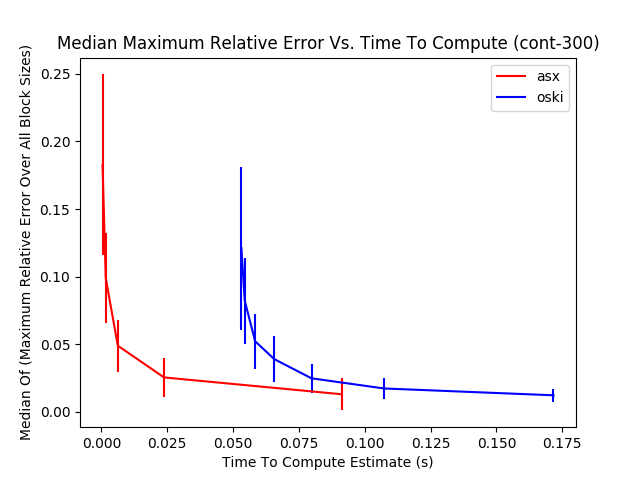
\includegraphics[width=1.0\linewidth]{../code/roi_cont-300.png}
    \caption{Results on a matrix}
    \label{fig:sub1}
  \end{subfigure}%
  \begin{subfigure}{.5\textwidth}
    \centering
    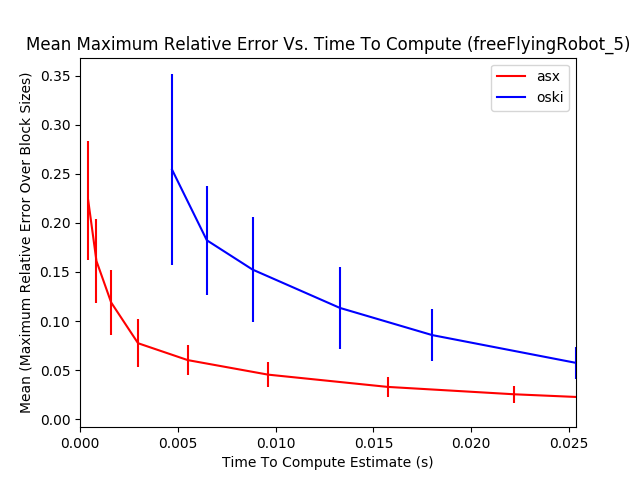
\includegraphics[width=1.0\linewidth]{../code/roi_freeFlyingRobot_5.png}
    \caption{Results on a different matrix}
    \label{fig:sub2}
  \end{subfigure}
  \caption{Our results}
  \label{fig:test}
  \end{figure}

  Because oski samples entire rows, its accuracy and runtime depend on the shape of the matrix. Therefore, we compare the performance of asx and oski on a short fat matrix ($512 \times 8192$), a square matrix ($2048 \times 2048$), and a tall, skinny matrix ($8192 \times 512$) where nonzeros are randomly included with probability $1/12$. 


  \verb|http://www.math.sci.hiroshima-u.ac.jp/~m-mat/MT/MT2002/emt19937ar.html|


\end{document}
